\section{Theorie}
\label{sec:theorie}

    Im folgenden Abschnitt werden die theoretischen Grundlagen des Versuchs erläutert.

\subsection{Energieniveaus und Quantenzahlen eines Atoms}
\label{sec:energieaufspaltung}

    Bei der Betrachtung eines Atoms ist es sinnvoll,
    zwischen Kern und Atomhülle zu unterscheiden.

    Die Atomhülle besitzt einen Gesamtdrehimpuls $\vec{J}$,
    welcher sich aus dem Bahndrehimpuls $\vec{L}$ und dem Spin $\vec{S}$ der sich in der Hülle befindenden Elektronen zusammensetzt.
    Zu jedem dieser Drehimpulse gehört außerdem ein magnetisches Moment,
    welches durch
    \begin{gather*}
        \vec{\mu}_J = -g_J \mu_\text{B} \vec{J} \\
        \vec{\mu}_L = -g_L \mu_\text{B} \vec{L} \\
        \vec{\mu}_S = -g_S \mu_\text{B} \vec{S}
    \end{gather*}
    beschrieben werden kann,
    wobei $g_L = 1$ und $g_S \approx 2$ ist.
    Der Faktor $\mu_\text{B} = \frac{e \hbar}{2m_\text{e}}$ bezeichnet das Bohr'sche Magneton und $g_J$ stellt den Landé-Faktor der Elektronenhülle dar,
    welcher mit
    \begin{equation}
        g_J = 1 + \frac{J(J+1) + S(S+1) - L(L+1)}{2J(J+1)}
        \label{eqn:landeJ}
    \end{equation}
    berechnet werden kann.

    Die Elektronenkonfiguration innerhalb der Atomhülle kann über die Quantenzahlen $n, l, m$ beschrieben werden,
    wobei $n \in \symbb{N}$ die Energie- oder Hauptquantenzahl,
    ${ l \in \{0, 1, 2, \ldots, n-1\} }$ die Bahndrehimpulsquantenzahl und ${ m \in \{-l, -l+1, \ldots, l-1, l\} }$ die magnetische Quantenzahl ist.
    Das hier betrachtete Rubidium hat eine Elektronenkonfiguration von
    \[
        \ce{1s^2 \, 2s^2 \, 2p^6 \, 3s^2 \, 3p^6 \, 3d^10 \, 4s^2 \, 4p^6 \, 5s} \ .
    \]
    Wie jedes Alkali-Metall hat Rubidium ein einzelnes Valenzelektron in der äußersten Schale,
    welches alleinig zum Drehimpuls der Hülle beiträgt.
    Mithilfe der Hund'schen Regeln kann ein Gesamtspin von $S = \sfrac{1}{2}$,
    ein Gesamtbahndrehimpuls $L=0$ und ein Gesamtdrehimpuls von $J = \lvert L \pm S \rvert = \sfrac{1}{2}$ für die Atomhülle berechnet werden.

    Aufgrund der Wechselwirkung der magnetischen Momente von Spin $\vec{\mu}_S$ und Bahndrehimpuls $\vec{\mu}_L$ mit dem Magnetfeld des Kerns entsteht eine Aufspaltung der Energieniveaus,
    welche als \textit{Feinstrukturaufspaltung} oder \textit{LS-Kopplung} bezeichnet wird.

    Der Kern hat den Spin $\vec{I}$.
    Im Falle von \Rb{85} ergibt sich ein Spin von $I = \sfrac{5}{2}$ und für \Rb{87} gilt $I = \sfrac{3}{2}$.
    Der Spin lässt sich mithilfe der Spinkonfiguration von Protonen und Neutronen bestimmen.
    Mit Betrachtung des Kernspins tritt ein weiterer Effekt bei der Aufspaltung der Energieniveaus auf,
    die sogenannte \textit{Hyperfeinstruktur},
    welche aus der Wechselwirkung der magnetischen Momente des Kernspins $\vec{\mu}_I$ und dem des Gesamtbahndrehimpuls der Atomhülle $\vec{\mu}_J$ resultiert.

    Für das gesamte Atom ergibt sich ein Atomdrehimpuls $\vec{F} = \vec{I} + \vec{J}$ mit der magnetischen Quantenzahl $M = \{-\lvert I+J \rvert, \ldots, \lvert I+J \rvert\}$.
    Für das entsprechende magnetische Moment gilt
    \begin{equation}
        \vec{\mu}_F = - M g_F \mu_\text{B} \vec{F} \ ,
    \end{equation}
    %TODO: IST DIE GLEICHUNG SO RICHTIG?
    wobei
    \begin{equation}
        g_F = g_J \cdot \frac{F(F+1) + J(J+1) - I(I+1)}{2F(F+1)}
        \label{eqn:landeF}
    \end{equation}
    der Landé-Faktor des Atoms ist,
    mit $g_J$ aus \autoref{eqn:landeJ}.

    Beim Anlegen eines externen Magnetfelds wird der \textit{Zeeman-Effekt} relevant.
    Es findet eine Aufspaltung der Energieniveaus nach der magnetischen Quantenzahl $M$ statt,
    wodurch $2F+1$ Zustände entstehen und die Entartung der Niveaus in $M$ damit aufgehoben wird.
    Die Energiedifferenz zwischen diesen Zuständen wird mithilfe von
    \begin{equation}
        \symup{\Delta} E_\text{Z} = g_F \mu_\text{B} B \symup{\Delta} M
        \label{eqn:zeemanaufspaltung}
    \end{equation}
    berechnet.
    \autoref{fig:aufspaltung} zeigt die Feinstrukturaufspaltung,
    die Hyperfeinstrukturaufspaltung sowie die Aufspaltung durch den Zeeman-Effekt im Falle des zwei-Niveau-Systems mit Grundzustands $^2S_{1/2}$ und angeregtem Zustands $^2P_{1/2}$ von \Rb{87}.
    \begin{figure}[H]
        \centering
        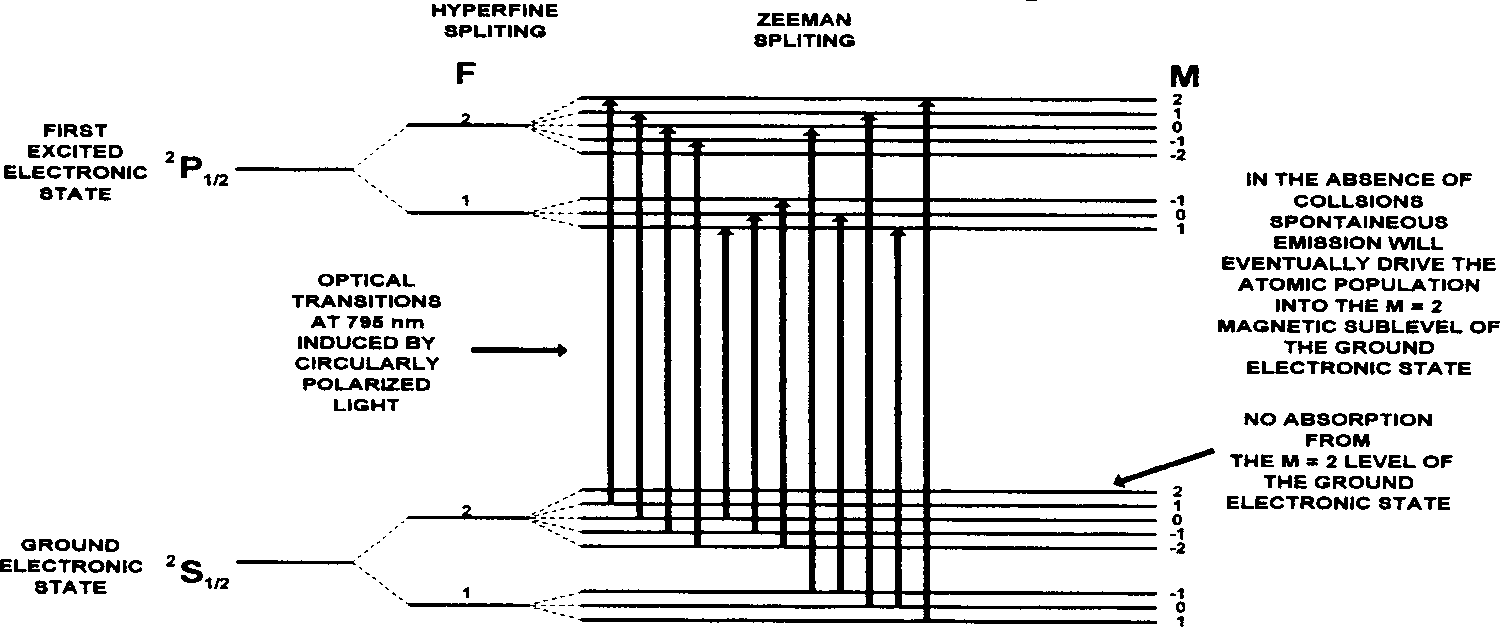
\includegraphics[width=\textwidth]{content/img/Lit2_Abb_2D-3.png}
        \caption{Aufspaltung der Energieniveaus durch Kopplungen innerhalb des Atoms und externe Magnetfelder. \cite{caltech}}
        \label{fig:aufspaltung}
    \end{figure}
    Zwischen den Energieniveaus können Übergänge stattfinden,
    allerdings nur solche,
    bei denen die Auswahlregeln für elektrische und magnetische Dipolübergänge erfüllt sind.
    Es gilt $\symup{\Delta} L = \pm 1$, $\symup{\Delta} S = 0$, $\symup{\Delta} J = 0, \pm 1$ und $\symup{\Delta} F = 0, \pm 1$.
    Entsprechend ergibt sich $\symup{\Delta} M = 0, \pm 1$.
    Abhängig davon,
    welchen Wert $\symup{\Delta} M$ bei einem Übergang annimmt,
    ist das entstehende Photon entweder linear ($\pi$-) polarisiert ($\symup{\Delta}M = 0$) oder zirkular ($\sigma^{\pm}$-) polarisiert ($\symup{\Delta}M = \pm 1$).
    Umgekehrt kann also nur ein $\sigma^{\pm}$-Übergang mit $\symup{\Delta} M = \pm 1$ stattfinden,
    wenn das Atom mit zirkular polarisiertem Licht bestrahlt wird.
    Dabei ist Licht mit $\symup{\Delta} M = +1$ rechts herum und Licht mit $\symup{\Delta} M =-1$ links herum polarisiert.

    Abhängig von der Feldstärke des angelegten Magnetfelds werden weitere Terme des Hamilton-Operator für die Energieaufspaltung beim Zeeman-Effekt relevant.
    Bei der hier verwendeten mittleren Feldstärke muss der \textit{quadratische Zeeman-Effekt} betrachtet werden.
    In diesem Fall ergibt sich mithilfe von Störungstheorie ein Energieterm der Gestalt
    \begin{equation}
        \symup{\Delta} E_\text{Z} = g_f \mu_\text{B} B + g^2_F \mu^2_\text{B} B^2 \frac{1 - 2M}{\symup{\Delta}E_\text{Hfs}} \ ,
        \label{eqn:quadr_zeeman}
    \end{equation}
    wobei $\symup{\Delta}E_\text{Hfs}$ die Energiedifferenz zwischen den aufgespaltenen Energienievaus der Hyperfeinstruktur beschreibt.


\subsection{Das optische Pumpen}
\label{sec:optisches_pumpen}

    Die Grundlage des optischen Pumpens ist durch die Absorption von Photonen in einem Atom gegeben,
    wenn das einfallende Licht mit der Energiedifferenz und den in \autoref{sec:energieaufspaltung} genannten Auswahlregeln kompatibel ist.
    Aufgrunddessen entsteht eine Besetzungsinversion im Atom.
    Es wird zusätzlich zwischen \textit{spontaner} und \textit{stimulierter Emission} unterschieden.
    Bei der spontanen Emission wird ein Photon beim Rückfall eines Atoms aus einem angeregten Zustand in den Grundzustand erzeugt.
    Die Wahrscheinlichkeit für einen Übergang durch spontane Emission ist durch den Einstein-Koeffizienten $A_{nm}$ gegeben,
    wobei die Indizes $nm$ die Energieniveaus $E_n$ und $E_m$ bezeichnen.
    Außerdem ist die Wahrscheinlichkeit der spontanen Emission $\propto \nu^3$,
    wobei $\nu$ die Frequenz des emittierten Photons beschreibt,
    was dazu führt,
    dass Übergänge mit einer größeren Energiedifferenz wahrscheinlicher sind.
    Bei der stimulierten Emission trifft ein Photon auf ein angeregtes Atom,
    welches daraufhin unter Aussendung von Photonen in den Grundzustand zurückfällt.
    Das einfallende und die emittierten Photonen sind dabei kohärent,
    haben also die gleiche Wellenlänge, Polarisation, Frequenz, Richtung und Phasenbeziehung.
    Die Übergangswahrscheinlichkeit ist durch den Einstein-Koeffizienten $B_{nm}$ gegeben.

    Es wird nun ein Zwei-Niveau-System mit dem Grundzustand $^2S_{1/2}$ und dem ersten angeregten Zustand $^2P_{1/2}$ betrachtet,
    wobei die Elektronen im thermischen Gleichgewicht nach der Boltzmann-Statistik verteilt sind.
    Der Übergang zwischen den beiden Niveaus wird als $D_1$ bezeichnet,
    die Energiedifferenz entspricht einer Wellenlänge von $\lambda = \SI{794.8}{\nano\meter}$ \cite{versuchsanleitung}.
    Wenn das System mit Licht dieser Wellenlänge,
    welches rechts herum polarisiert ist ($\symup{\Delta}M = +1$),
    bestrahlt wird,
    können solche Elektronen angeregt werden,
    für die ein Übergang mit $\symup{\Delta}M = +1$ möglich ist.
    Dies ist in \autoref{fig:aufspaltung} zu sehen.
    Wenn alle möglichen Absorptionsübergänge stattgefunden haben,
    kann keine weitere Absorption stattfinden,
    das Gas wird daher als \textit{transparent} bezeichnet.
    Die Elektronen können durch spontane oder stimulierte Emission wieder in den Grundzustand zurückkehren.
    Bei der spontanen Emission entstehen stochastisch verteilte Photonen,
    – es ist jede Konfiguration von $\symup{\Delta}M = 0, \pm 1$ möglich –
    während bei stimulierter Emission aufgrund der Kohärenzbedingung nur Übergänge mit $\symup{\Delta}M = +1$ erlaubt sind.

    Der gesamte Vorgang des optischen Pumpens ist in \autoref{fig:pumpen} dargestellt.
    \begin{figure}[H]
        \centering
        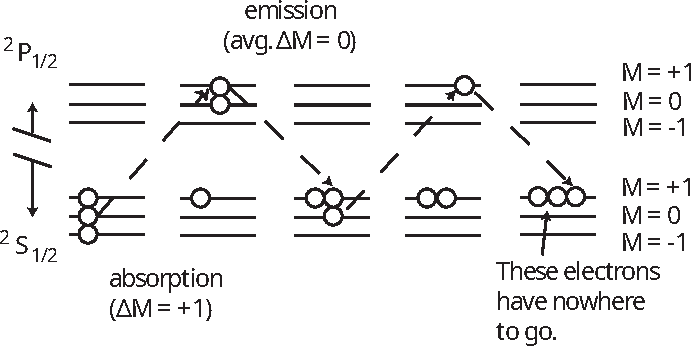
\includegraphics[scale=1]{content/img/Lit2_Abb_8.pdf}
        \caption{Übergänge im zwei-Niveau-System beim optischen Pumpen. \cite{caltech}}
        \label{fig:pumpen}
    \end{figure}

    Wird nun die angelegte Magentfeldstärke variiert,
    ergibt sich die Darstellung in \autoref{fig:transparenz}.
    Die Peaks entstehen bei einer Magnetfeldstärke $B_\text{m}$ dann,
    wenn die Frequenz des eingestrahlten Lichts einem der Übergänge entspricht,
    sodass es zu stimulierter Emission kommt und sich wieder mehr Elektronen im Grundzustand befinden.
    Für dieses Phänomen gilt die Beziehung
    \begin{align}
        E_\text{Rf} = \symup{\Delta} E_\text{Z} & \iff h \nu = \hbar \omega_\text{Rf} = g_F \mu_\text{B} B \symup{\Delta} M
        \
    \end{align}
    \begin{figure}
        \centering
        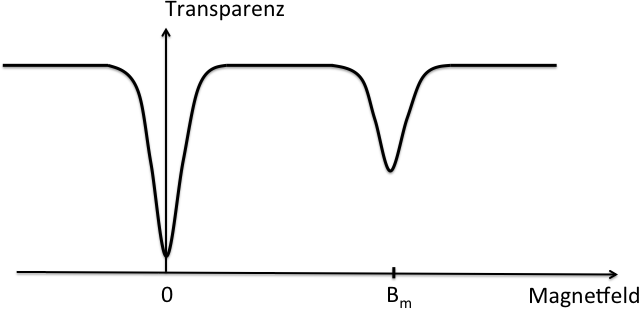
\includegraphics[scale=0.5]{content/img/Abb_2.png}
        \caption{Verlauf der Transparenz des Gases in Abhängigkeit der Magnetfeldstärke. \cite{versuchsanleitung}}
        \label{fig:transparenz}
    \end{figure}

    Dieser Effekt tritt auch auf,
    wenn kein Magnetfeld angelegt ist,
    also $B = 0$ gilt.
    In diesem Fall ist keine Aufspaltung in $M$ zu beobachten,
    die Photonen werden allerdings trotzdem absorbiert und können stimulierte Emission anregen.











